\documentclass[conference]{IEEEtran}

\usepackage{cite}
\usepackage{amsmath,amssymb,amsfonts}
\usepackage{graphicx}
\usepackage{booktabs}
\usepackage{array}
\usepackage{url}
\usepackage{xcolor}

\title{Notes on Adjusted R Squared}

\author{
\IEEEauthorblockN{Luis Mendez}
}

\begin{document}

\maketitle

\section*{Adjusted R Squared}

Adjusted R Squared is a modified version of the R Squared metric that takes into account the number of predictors in a regression model.

\begin{figure}[htbp]
    \centering
    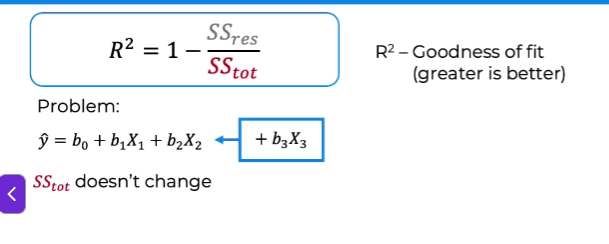
\includegraphics[width=0.75\linewidth]{image.png}
    \caption{Illustration of Adjusted $R^2$.}
    \label{fig:adjusted_r2}
\end{figure}

It is calculated using the formula:

\[
\text{Adjusted } R^2 =
1 - \left(
\frac{(1 - R^2)(n - 1)}
     {n - k - 1}
\right)
\]

where:

\begin{itemize}
    \item $R^2$ is the coefficient of determination (R Squared),
    \item $n$ is the number of observations,
    \item $k$ is the number of predictors in the model.
\end{itemize}

The Adjusted R Squared value can be negative if the model fits the data very poorly. Unlike regular $R^2$, which always increases when additional predictors are added, Adjusted $R^2$ penalizes the inclusion of unnecessary variables.

A higher Adjusted $R^2$ generally indicates a better-fitting model, while a lower value suggests that the predictors do not explain the variation in the response variable effectively. This makes Adjusted $R^2$ useful for comparing regression models that contain different numbers of predictors.

However, Adjusted $R^2$ should not be the only criterion used for model selection. Statistical significance tests, residual analysis, and domain-specific considerations should also be taken into account when evaluating model performance.

If $SS_{tot}$ doesn't change, then the Adjusted R Squared will decrease as more predictors are added, which is a key reason why it is preferred over regular R Squared for model comparison.
If $SS_{res}$ will decrease or stay the same as more predictors are added, but the Adjusted R Squared will only increase if the new predictor improves the model sufficiently to offset the penalty for adding more predictors. (This is because of Ordinary Least Squares: $SS_{res} \to \min$)

\end{document}